\documentclass{beamer}
%\usepackage[dutch]{babel}
\usepackage[utf8]{inputenc}
\usepackage[T1]{fontenc}
\usepackage{amsmath}
\usepackage{amssymb}
\usepackage[makeroom]{cancel}
\usepackage{color}
\usepackage{color}
\useoutertheme{default}
\newcommand<>{\xxcancel}[1]{\alt#2{\cancel{#1}\vphantom{#1}}{#1}} %has apparently no effect
%\renewcommand{\CancelColor}{blue}

\newcommand{\C}{\ensuremath{\mathbb{C}}}
\newcommand{\N}{\ensuremath{\mathbb{N}}}
\newcommand{\E}{\ensuremath{\mathbb{E}}}
\newcommand{\norm}[1]{\left\|#1\right\|} % commando's met argumenten
\newcommand{\pa}[2]{\frac{\partial #1}{\partial #2}}
\newcommand{\ppa}[2]{\frac{\partial^2 #1}{\partial #2^2}}
\newcommand{\dd}{\ensuremath{\mathrm{d}}}
\newcommand{\U}{\ensuremath{\boldsymbol{\rho}}}
\newcommand{\cts}{\ensuremath{\boldsymbol{\Phi}_T}} %Coarse time step
\newcommand{\V}{\ensuremath{\mathbf{v}}}
\newcommand{\jv}{\ensuremath{\mathbf{\hat{Jv}}}}
\newcommand{\jvpde}{\ensuremath{\mathbf{Jv}_{FP}}}

\begin{document}



\title[Systemic Risk] % (optional, only for long titles)
{Variance Reduction in Equation-free Newton-Krylov-Methods}
%\subtitle{Evidence from India}
%\author[Author, Anders] % (optional, for multiple authors)
%{F.~Author\inst{1} \and S.~Anders\inst{2}}
%\institute[Universities Here and There] % (optional)
%{
%  \inst{1}%
%  Institute of Computer Science\\
%  University Here
%  \and
%  \inst{2}%
%  Institute of Theoretical Philosophy\\
%  University There
%}
\date{July 12, 2016} % (optional)
%{Conference on Presentation Techniques, 2004}
%\subject{Computer Science}

\begin{frame}{\titlepage}
\includegraphics[width=0.63\paperwidth,height=0.42\paperheight]{/home/pieter/riskmodel/domino-effect2}
%\includegraphics[width=0.6\paperwidth,height=0.53\paperheight]{/home/pieter/riskmodel/domino-effect3}
\end{frame}

\tableofcontents


\section{Model Problem}

\begin{frame}
\frametitle{Fokker-Planck equation}

\begin{equation*}
\label{fokkerplanck}
\pa{\rho(x,t)}{t} + \pa{(\mu(x) \rho(x,t))}{x} = \frac{\sigma^2}{2}  \ppa{\rho(x,t)}{x} 
\end{equation*}
%\begin{center}
%%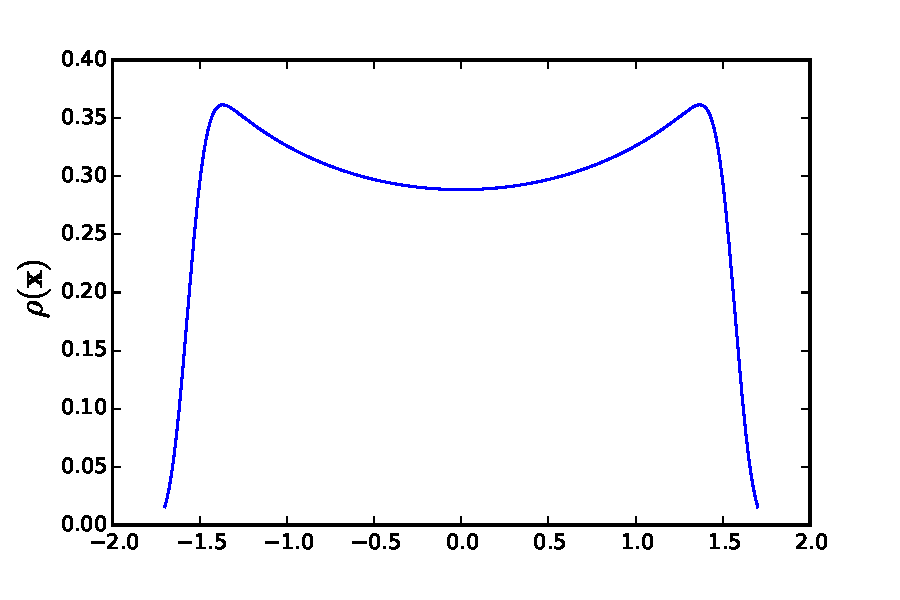
\includegraphics[width=6.5cm]{../Problems/WeightedParticles/checkSystem/plots/rho_pde}
%\end{center}


Simulate an ensemble of $N$ particles evolving according to the corresponding SDE
\begin{equation*}
    \dd X = \mu f(X) \dd t + \sigma  \dd{W_t}.
\end{equation*}

\end{frame}

\begin{frame}

\frametitle{Coarse time stepper}

\begin{equation*}
\U(t + n \Delta t) = \cts(\U) = (\mathcal{R} \circ \mathcal{E}(n \Delta t, \omega) \circ  \mathcal{L}(\mathbf{\omega})  ) (\U(t))
\end{equation*}


\begin{itemize} [<+->]
\item 
\begin{block} 
{Lifting $\mathcal{L}: \U \rightarrow \mathbf{x}  $}
\end{block}
\item
 \begin{block} {Evolution  $\mathcal{E}$: \\ Simulation of the SDE for $N$ particles over $n$ timesteps. }
\begin{equation*}
   \mathbf{X}^{n + 1} = \mathbf{X}^{n} + \mu (\mathbf{X}^n) \Delta t +  \sqrt{\sigma \Delta t}\cdot \boldsymbol{\xi}^n 
\end{equation*}
with \begin{equation*}\xi^n(\omega)  \sim \mathcal{N} (0,1)
\end{equation*}
\end{block}

\item 
\begin{block} {Restriction $\mathcal{R}: \mathbf{x} \rightarrow \U $}
\begin{equation*}
\frac{1}{N} \sum_{i=1}^{N}  w_i \cdot \chi_{\Delta_j}(X_i) = \rho_j  
\end{equation*}
\end{block}

\end{itemize}

\end{frame}



\begin{frame}
\frametitle{Evaluating the bias on Jacobian-vector products}


\begin{equation*} 
 \mathbf{Bias}(\jv, \jvpde ) = \mathbb{\hat{E}}[\jv]  - \jvpde 
\end{equation*}





\pause 

with 
\begin{equation*}
\jvpde \approx \frac{ \U^{\varepsilon}(t + n \Delta t)  - \U (t +  n\Delta t)}{\varepsilon}
\end{equation*}
 \pause 

and $\U$ calculated by explicitly solving 

\begin{equation*}
\label{fokkerplanck}
\pa{\rho(x,t)}{t} + \pa{(\mu(x) \rho(x,t))}{x} = D  \ppa{\rho(x,t)}{x} 
\end{equation*}

 using

\begin{equation*} 
\rho_i^{n+1} = \rho_i^n + \Delta t \left( \frac{D}{{\Delta x}^2} \left( \rho_{i+1}^{n} - 2 \rho_i^n + \rho_{i-1}^n \right)  - \frac{a(x)}{\Delta x} (\rho_i^n - \rho_{i-1}^n) \right)
\end{equation*}
for the value of $\rho$ at position $x=i \Delta x$ and time $t=(n+1) \Delta t$

\end{frame}

\begin{frame}
\frametitle{Evaluating the bias on Jacobian-vector products}


\begin{equation*} 
 \mathbf{Bias}(\jv, \jvpde ) = \mathbb{\hat{E}}[\jv]  - \jvpde 
\end{equation*}

 
 \begin{figure}
 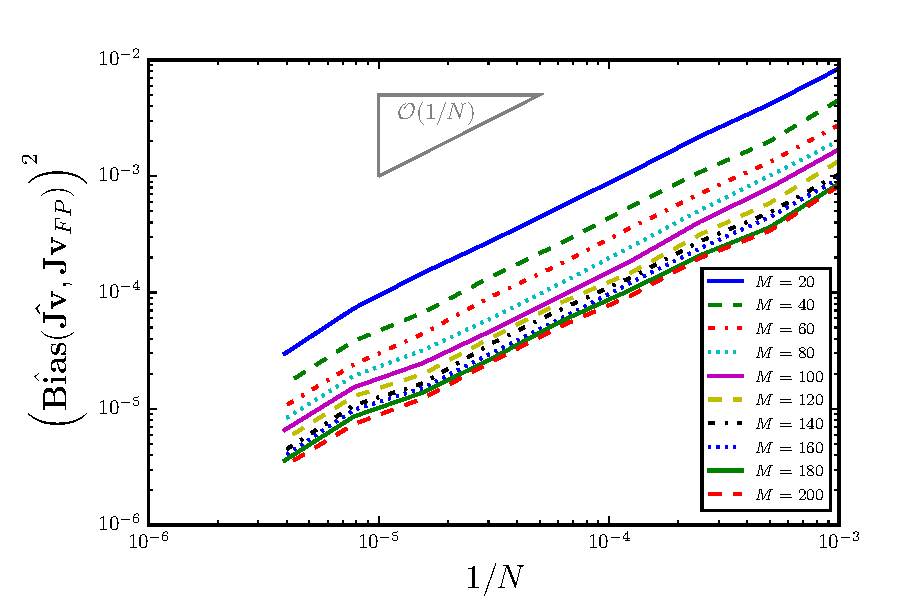
\includegraphics[width=9.5cm]{../Problems/WeightedParticles/checkSystem/plots/Bias_Jv_N_M.pdf}

 \end{figure}

\end{frame}



\begin{frame}
\frametitle{Evaluating the bias on Jacobian-vector products}


\begin{equation*} 
 \mathbf{Bias}(\jv, \jvpde ) = \mathbb{\hat{E}}[\jv]  - \jvpde 
\end{equation*}
 
 \begin{figure}
 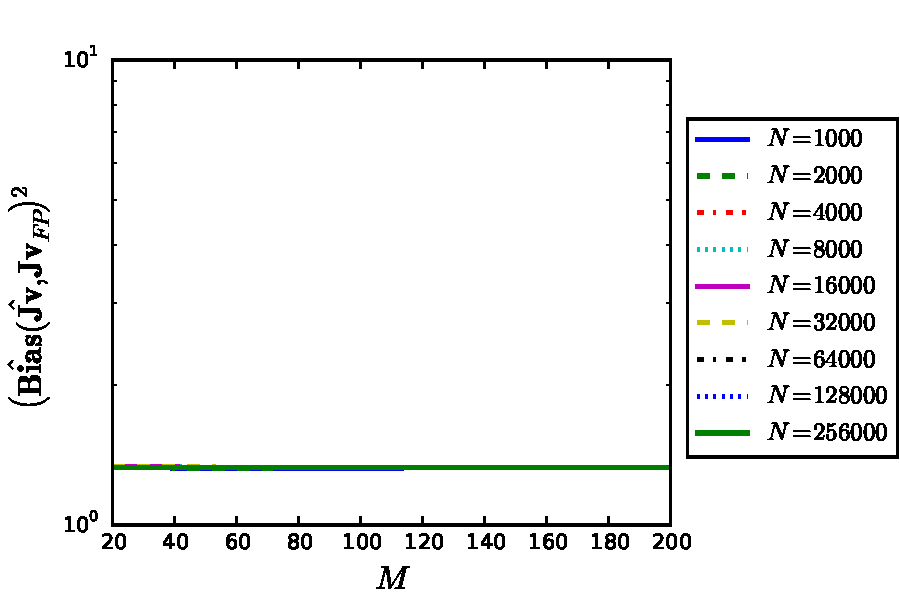
\includegraphics[width=9.5cm]{../Problems/WeightedParticles/checkSystem/plots/Bias_Jv_M_N.pdf}

 \end{figure}

\end{frame}



\section{Algorithm}

\begin{frame} {Newton-Krylov solver}


Computing steady states $\U^*$ by solving the non-linear system

\begin{equation*}
  {F}(\U^*) = \U^* - \cts(\U^*) =0 \label{non-linear_system}
\end{equation*}

\pause
%where $\mathbf{F}$ is nonlinear function from $\R^N$ to  $\R^N$. 
%To find the steady state $\U_*$, we apply Newton's method to eq. \ref{non-linear_system} . Starting from an initial state $\U^0$, 
\begin{itemize}
\item Starting from an initial state $\U^0$, we iterate
\begin{eqnarray*}
\begin{cases}
& \texttt{Solve         }  J(\U^k) \boldsymbol{\delta_k}  =  - {F}(\U^k) \label{linear_system}        \\          
& \texttt{Set     } \U^{k+1} = \U^k+ \boldsymbol{\delta_k} 
\end{cases}
\end{eqnarray*}
until convergence


\pause

%\item Each Newton iteration $n$ involves evaluating the Jacobian of the timestepper $J(\cts(\U))$
\item  No explicit formula for $J(\cts)$ $\Rightarrow$ using iterative method (GMRES) that only requires Jacobian-vector products


\pause
\item  These are estimated by a finite difference approximation


\begin{equation*}
\label{Jv_approx}
J(\cts) \cdot \mathbf{v} \approx \frac{\cts (\U + \varepsilon \mathbf{v}, \boldsymbol{\omega_1} )  - \cts (\U, \boldsymbol{\omega_2})}{\varepsilon} 
%&\approx & \frac{\cts (\U, \boldsymbol{\omega_1} )  + \varepsilon D(\cts) (  \U, \boldsymbol{\omega_1})  \cdot \mathbf{v}  - \cts (\U, \boldsymbol{\omega_2}) }{\varepsilon} \nonumber
\end{equation*}

%\pause
%\item Problem: $ \texttt{Var}(\jv)  \sim \mathcal{O}(1/(\varepsilon^2  N)) $\\$ \Rightarrow $     Numerical noise for $ \varepsilon \ll 1$    
%%\end{frame}
%\end{itemize}


\pause
\begin{block}{Problem}
 $ \texttt{Var}(\jv)  \sim \mathcal{O}(1/(\varepsilon^2  N)) \Rightarrow $     Numerical noise for $ \varepsilon \ll 1$ 
 \end{block}  
%\end{frame}
\end{itemize}
\end{frame}
%
%\begin{frame} \frametitle{Variance reduction of Jacobian-vector products}
%
%\begin{equation*}
%\label{Jv_approx}
%J(\cts) \cdot \mathbf{v} \approx \frac{\cts (\U + \varepsilon \mathbf{v}, \boldsymbol{\omega_1} )  - \cts (\U, \boldsymbol{\omega_2})}{\varepsilon} 
%%&\approx & \frac{\cts (\U, \boldsymbol{\omega_1} )  + \varepsilon D(\cts) (  \U, \boldsymbol{\omega_1})  \cdot \mathbf{v}  - \cts (\U, \boldsymbol{\omega_2}) }{\varepsilon} \nonumber
%\end{equation*}
%Problem: $ \texttt{Var}(\jv)  \sim \mathcal{O}(1/(\varepsilon^2  N)) \Rightarrow $ 
%    Numerical noise for $ \varepsilon \ll 1$    
%\end{frame}
%

\begin{frame} \frametitle{Variance reduction of Jacobian-vector products}

\begin{eqnarray}
\mathbf{Jv} = D(\cts) \cdot \mathbf{v} &\approx& \frac{\cts (\U + \varepsilon \mathbf{v}, \boldsymbol{\omega_1} )  - \cts (\U, \boldsymbol{\omega_2})}{\varepsilon} \nonumber \\
&\approx & \frac{\cts (\U, \boldsymbol{\omega_1} )  + \varepsilon D(\cts) (  \U, \boldsymbol{\omega_1})  \cdot \mathbf{v}  - \cts (\U, \boldsymbol{\omega_2}) }{\varepsilon} \nonumber
\end{eqnarray}



\pause 
\begin{block}{Solution: \\ Perturbations on the density $\rightarrow$  perturbations in the weights }
\begin{eqnarray*}
\frac{1}{N} \sum_{i=1}^{N}  w_i \cdot \chi_{\Delta_j}(x_i) &=& \rho_j  \\
\frac{1}{N} \sum_{i=1}^{N}  w^i_{\varepsilon} \cdot \chi_{\Delta_j} (x^i) &=& \rho_j + \varepsilon v_j .
\end{eqnarray*}
For the perturbated density: compute the weight per bin as $ w^j_{\varepsilon} = 1+ \frac{\varepsilon v_j}{\rho_j}$ and assign this value to each particle in $\Delta_j$.
\end{block}


\end{frame}

\begin{frame} \frametitle{Variance reduction of Jacobian-vector products}

\begin{eqnarray}
\mathbf{Jv} = D(\cts) \cdot \mathbf{v} &\approx& \frac{\cts (\U + \varepsilon \mathbf{v}, \boldsymbol{\omega_1} )  - \cts (\U, \boldsymbol{\omega_2})}{\varepsilon} \nonumber \\
&\approx &  \frac{ \cancel{\cts (\U, \boldsymbol{\omega_1} ) }  + \varepsilon D(\cts) (  \U, \boldsymbol{\omega_1})  \cdot \mathbf{v}  - \cancel{ \cts (\U, \boldsymbol{\omega_1}) } }{\varepsilon} \nonumber
\end{eqnarray}

\begin{block}{Solution: \\ Perturbations on the density $\rightarrow$  perturbations in the weights }
\begin{eqnarray*}
\frac{1}{N} \sum_{i=1}^{N}  w_i \cdot \chi_{\Delta_j}(x_i) &=& \rho_j  \\
\frac{1}{N} \sum_{i=1}^{N}  w^i_{\varepsilon} \cdot \chi_{\Delta_j} (x^i) &=& \rho_j + \varepsilon v_j .
\end{eqnarray*}
For the perturbated density: compute the weight per bin as $ w^j_{\varepsilon} = 1+ \frac{\varepsilon v_j}{\rho_j}$ and assign this value to each particle in $\Delta_j$.
\end{block}

\end{frame}

\begin{frame} \frametitle{Variance reduction of Jacobian-vector products}

\begin{eqnarray}
\mathbf{Jv} = D(\cts) \cdot \mathbf{v} &\approx& \frac{\cts (\U + \varepsilon \mathbf{v}, \boldsymbol{\omega_1} )  - \cts (\U, \boldsymbol{\omega_2})}{\varepsilon} \nonumber \\
&\approx &  \frac{ \xxcancel{\cts (\U, \boldsymbol{\omega_1} ) }  + \varepsilon D(\cts) (  \U, \boldsymbol{\omega_1})  \cdot \mathbf{v}  - \xxcancel{ \cts (\U, \boldsymbol{\omega_1}) } }{\varepsilon} \nonumber
\end{eqnarray}

\begin{block}{Solution: \\ Perturbations on the density $\rightarrow$  perturbations in the weights }
\begin{eqnarray*}
\frac{1}{N} \sum_{i=1}^{N}  w_i \cdot \chi_{\Delta_j}(x_i) &=& \rho_j  \\
\frac{1}{N} \sum_{i=1}^{N}  w^i_{\varepsilon} \cdot \chi_{\Delta_j} (x^i) &=& \rho_j + \varepsilon v_j .
\end{eqnarray*}
For the perturbated density: compute the weight per bin as $ w^j_{\varepsilon} = 1+ \frac{\varepsilon v_j}{\rho_j}$ and assign this value to each particle in $\Delta_j$.
\end{block}
\end{frame}


\begin{frame} \frametitle{Variance reduction of Jacobian-vector products}

\begin{eqnarray}
\mathbf{Jv} = D(\cts) \cdot \mathbf{v} &\approx& \frac{\cts (\U + \varepsilon \mathbf{v}, \boldsymbol{\omega_1} )  - \cts (\U, \boldsymbol{\omega_2})}{\varepsilon} \nonumber \\
&\approx &  \frac{ \xxcancel{\cts (\U, \boldsymbol{\omega_1} ) }  + \xxcancel{\varepsilon} D(\cts) (  \U, \boldsymbol{\omega_1})  \cdot \mathbf{v}  - \xxcancel{ \cts (\U, \boldsymbol{\omega_1}) } }{\xxcancel{\varepsilon}} \nonumber
\end{eqnarray}

\begin{block}{Solution: \\ Perturbations on the density $\rightarrow$  perturbations in the weights }
\begin{eqnarray*}
\frac{1}{N} \sum_{i=1}^{N}  w_i \cdot \chi_{\Delta_j}(x_i) &=& \rho_j  \\
\frac{1}{N} \sum_{i=1}^{N}  w^i_{\varepsilon} \cdot \chi_{\Delta_j} (x^i) &=& \rho_j + \varepsilon v_j .
\end{eqnarray*}
For the perturbated density: compute the weight per bin as $ w^j_{\varepsilon} = 1+ \frac{\varepsilon v_j}{\rho_j}$ and assign this value to each particle in $\Delta_j$.
\end{block}
\end{frame}


\begin{frame}
\frametitle{Variance reduction of Jacobian-vector products}

\begin{equation*} 
 \texttt{Var}(\jv) =  \hat{\mathbb{E}} \left[   \left(  \jv - \hat{\mathbb{E}}[\jv]   \right)^2 \right] \sim \mathcal{O}(1/ N)
\end{equation*}

\begin{figure}
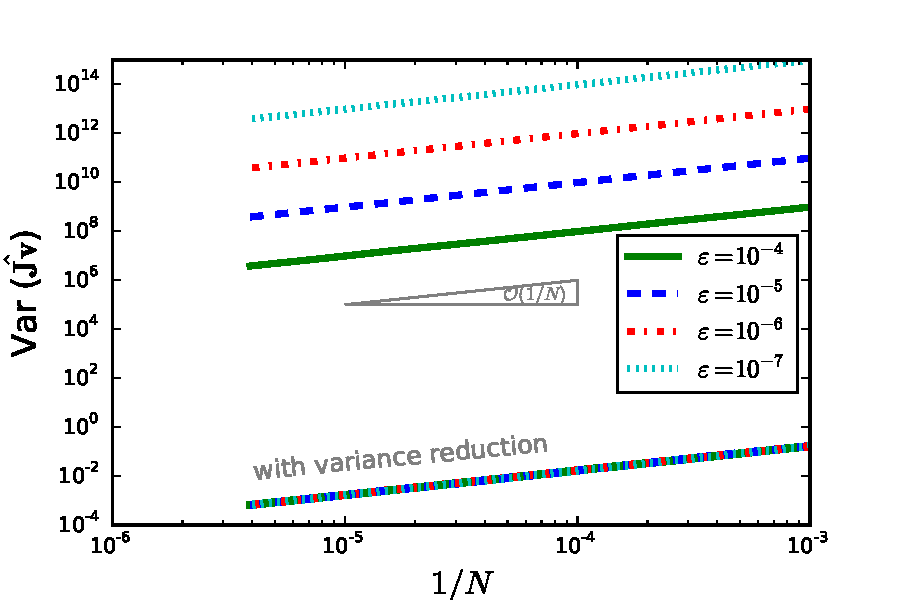
\includegraphics[width=8cm]{../Problems/Particles/checkSystem/plots/Var_N_eps_nw}
\end{figure}

\end{frame}



\section{Systemic risk}




\begin{frame} {Mean Field Model}

\begin{block}{Interaction between components}
\begin{itemize} 
\item Adding \emph{mean field interaction} to model:  each particle feels an attractive force towards the mean state (each agent tends to follow the state of the majority) 
\begin{equation*} 
\label{SDE_meanfield}
    \dd X_j = \mu f(X_j) \dd t + \sigma  \dd{W_j} + \alpha(\bar{X} -X_j) \dd t 
\end{equation*}
\item Interconnectedness between agents can affect the stability of the whole system %, causing systemic risk 
\end{itemize}
\end{block}

\pause

\begin{block}{Application: Systemic Risk in Banking Systems}
\begin{itemize}
\item Banks cooperate. By spreading the risk of
credit shocks, they try to minimize their own risk.
\item  However, this increases the  risk that they may all fail 
\end{itemize}
\end{block}

\end{frame}



\begin{frame} {Mathematical Model for Systemic Risk}

\begin{equation*} 
\label{SDE_meanfield}
    \dd X_j = \mu f(X_j) \dd t + \sigma  \dd{W_j} + \alpha(\bar{X} -X_j) \dd t 
\end{equation*}

\begin{itemize}
\item $\mu$ The intrinsic stability of each component
\item $\sigma$ The strength of external random perturbations to the system
\item $\alpha$ The degree of interconnectedness between agents
\end{itemize}

\begin{figure}
\centering
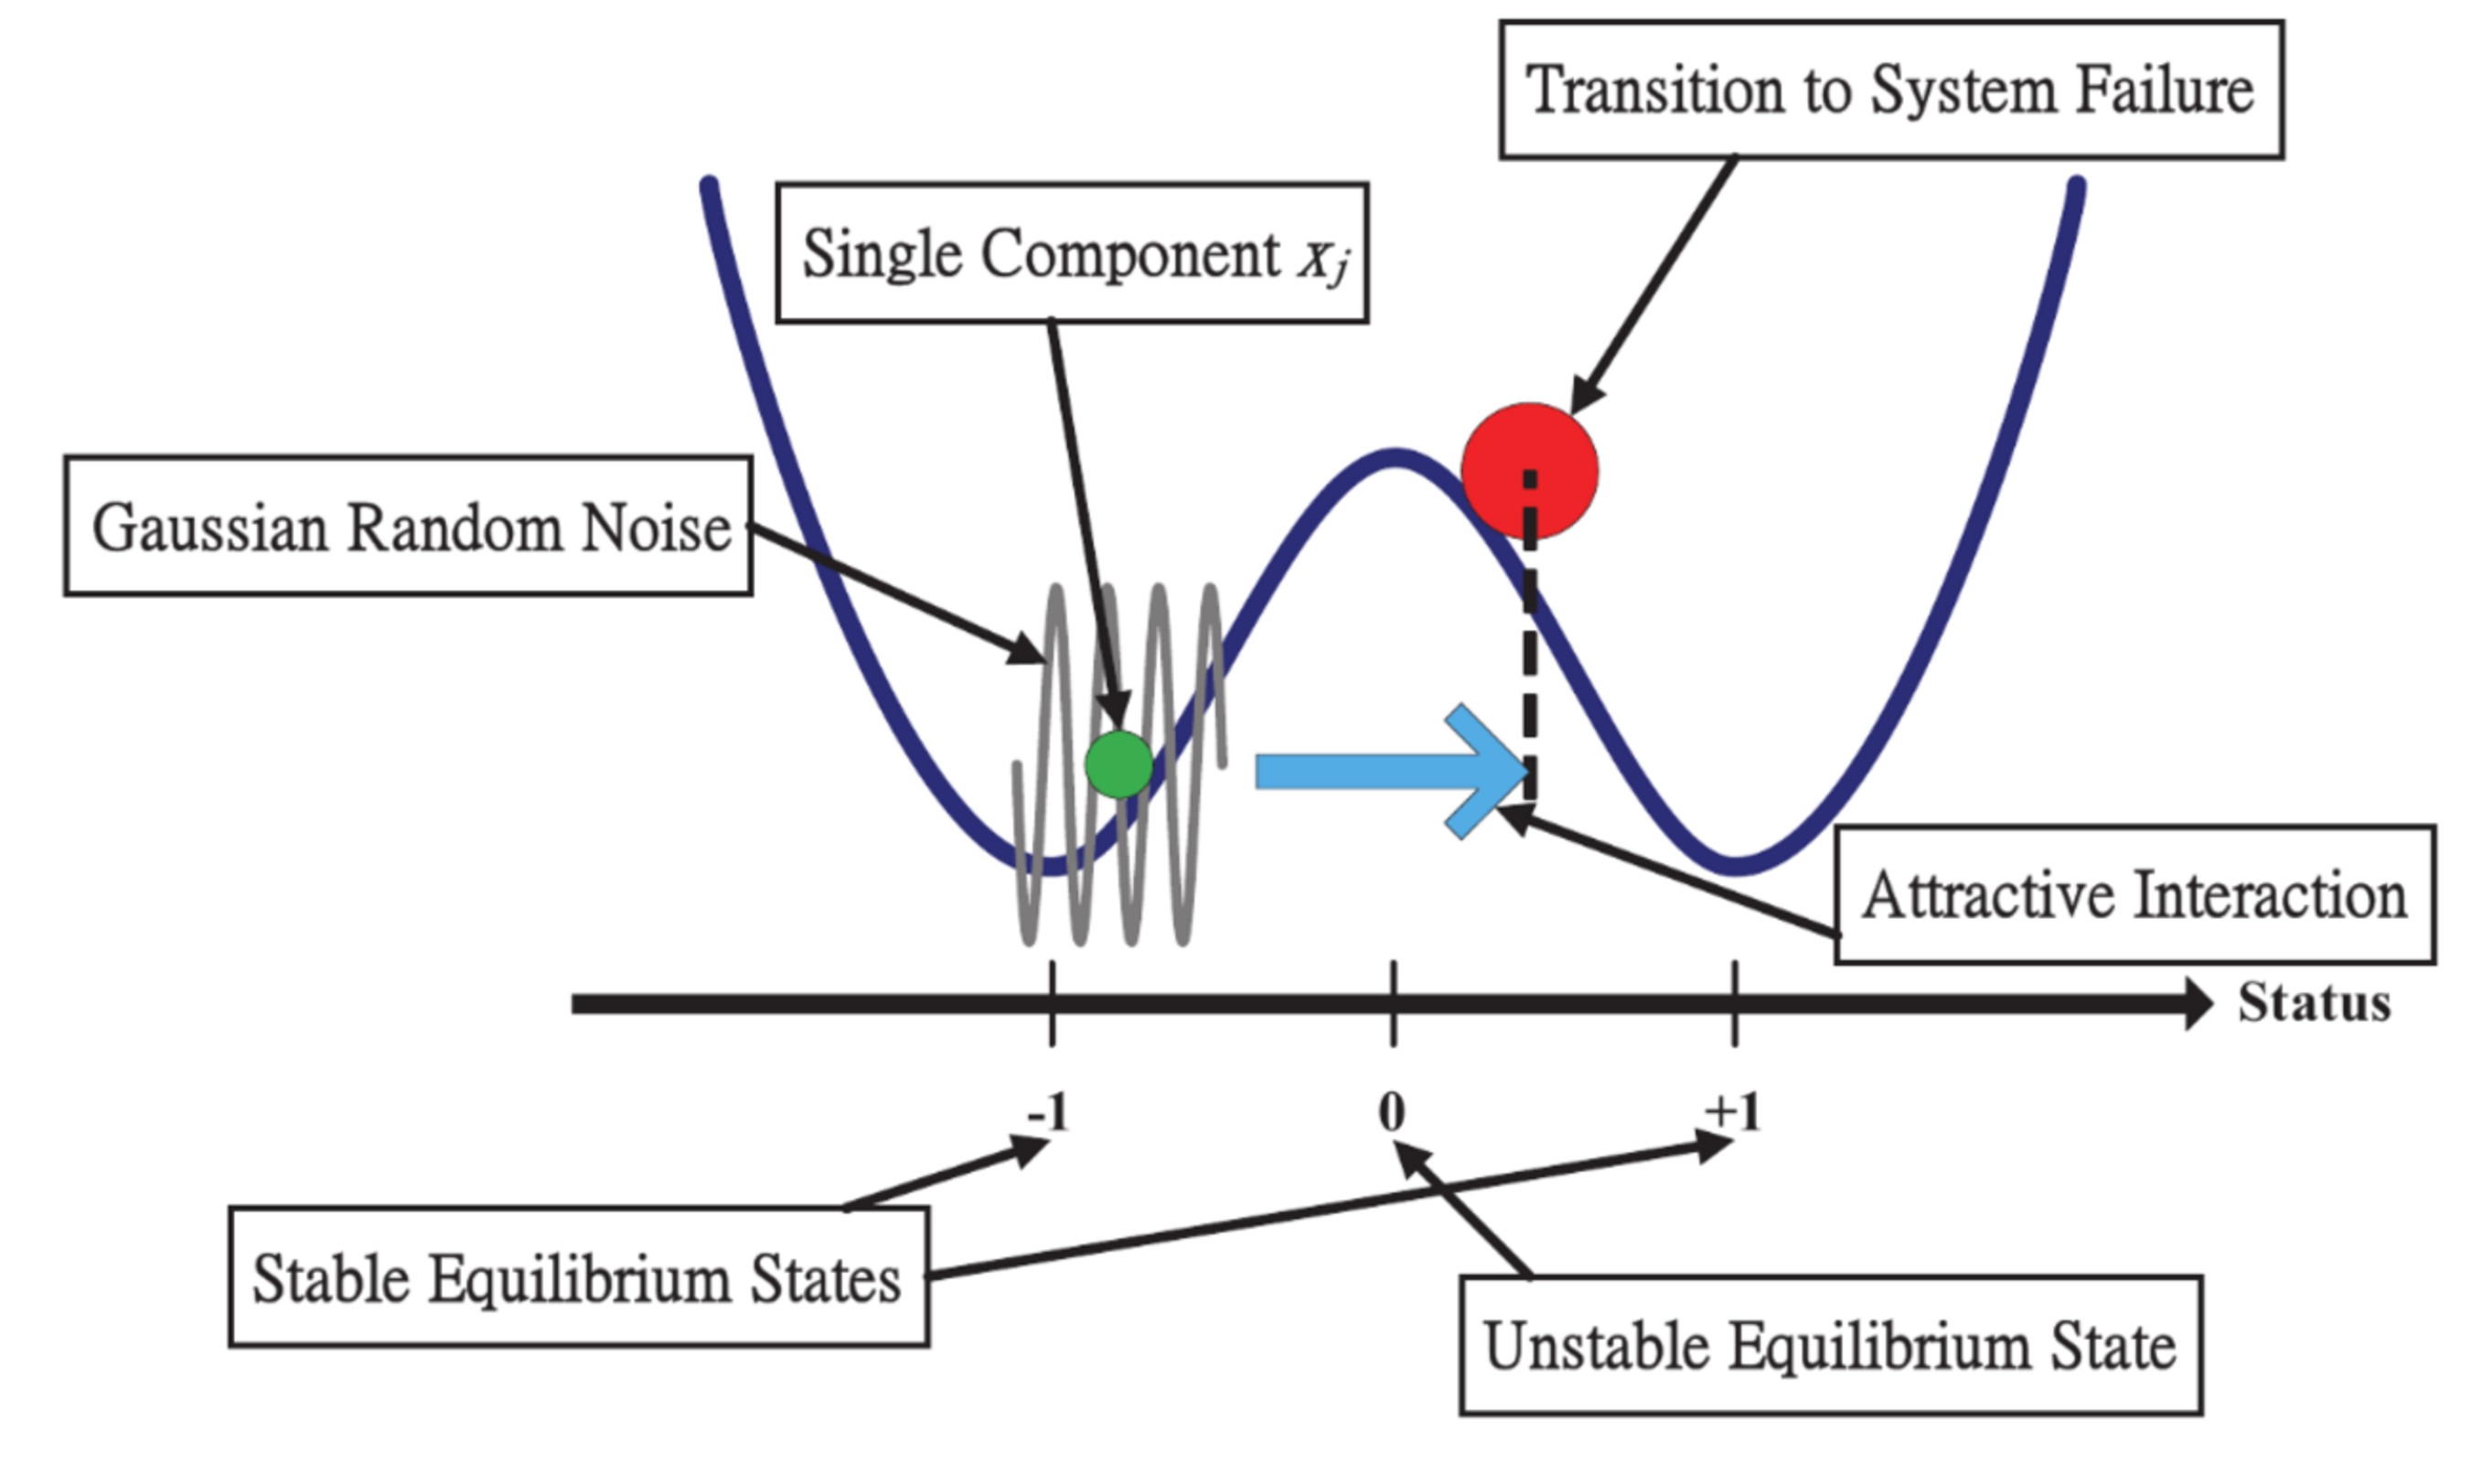
\includegraphics[width=0.8\linewidth]{./Risk_potential_cartoon}
\label{fig:Risk_potential_cartoon}
\end{figure}

%
%\end{itemize}

\end{frame}



\begin{frame} {Metastable Coarse States}


% \item Strength of mean field interaction $\alpha$ = bifurcation parameter
\begin{minipage}{1\textwidth}
\includegraphics[width=0.53\linewidth]{/home/pieter/riskmodel/Problems/WeightedParticles/checkSystem/plots/xmean_alpha1}
\includegraphics[width=0.53\linewidth]{/home/pieter/riskmodel/Problems/WeightedParticles/checkSystem/plots/xmean_alpha5}
\end{minipage}
\pause
%Upon increasing interaction strength $\alpha$, two metastable coarse states arise %$\rightarrow$ two new macroscopic states
\begin{figure}
\centering
\includegraphics[width=0.52\linewidth]{/home/pieter/riskmodel/Problems/WeightedParticles/checkSystem/plots/bif_alpha}
\label{fig:bif_alpha}
\end{figure}


\end{frame}




\begin{frame}
\frametitle{Analytic Solution for Equilibrium Distribution}

\begin{equation*}
\label{fp_mean_field}
\pa{\rho}{t} = - \mu \pa{( f(x) \rho)}{x} - \alpha \pa{}{x} \left[ \left(\int x \rho \mathrm{d}x  -x \right) \rho \right]   + \frac{\sigma^2}{2}  \ppa{\rho }{x} .
\end{equation*}

\pause

Assuming that \(\xi = \lim_{t \to \infty} \int x \rho(x,t) \mathrm{d}x \), an equilibrium solution satisfies
\begin{equation*}
-\mu \pa{( f(x) \rho_{\xi}) }{x}   - \alpha \pa{}{x} \left [( \xi -x) \rho_{\xi}  \right] +\frac{\sigma^2}{2} \ppa{\rho_{\xi}}{x}=0
\end{equation*}

\pause
 
The non-zero solutions $\pm\xi$ are


\begin{equation*}
\xi = \pm \sqrt{1-3\frac{\sigma^2}{2\alpha}}\left(1+
\ \mu \frac{6}{\sigma^2}\left(\frac{\sigma^2}{2\alpha}\right)^2\frac{1-2\frac{\sigma^2}{2\alpha} }{1-3\frac{\sigma^2}{2\alpha}}\right) + \mathcal{O}(\mu^2)
\end{equation*}  


\end{frame}


\begin{frame} {Calculate fixed points by applying variance reduced Newton-Krylov-solver}



\begin{equation*}
  {F}(\U^*) = \U^* - \cts(\U^*) =0 \label{non-linear_system}
\end{equation*}
\begin{eqnarray*}
\begin{cases}
& \texttt{Solve         }  J(\U^k) \boldsymbol{\delta_k}  =  - {F}(\U^k) \label{linear_system}        \\          
& \texttt{Set     } \U^{k+1} = \U^k+ \boldsymbol{\delta_k} 
\end{cases}
\end{eqnarray*}

\pause


\begin{itemize}
\item How to choose the Newton tolerance?
\item Which time window to choose for the coarse time stepper \cts? 
\end{itemize}
\begin{figure}
\centering
\includegraphics[width=0.52\linewidth]{/home/pieter/riskmodel/Problems/WeightedParticles/checkSystem/plots/steady_states_upd}
\label{fig:steady_states}
\end{figure}




\end{frame}




\begin{frame} {Estimating Stopping Criterion for the Non-linear Solver}

\begin{itemize}

\item The accuracy on the Newton-Krylov solution is inevitably limited by the noise on the stochastic coarse-time-stepper

\item When the Newton-Krylov solution is
converged, it stays oscillating around the true solution with a standard deviation depending
on the number of particles.

\end{itemize}

\begin{figure}
\includegraphics[width=0.57\linewidth]{/home/pieter/riskmodel/Problems/WeightedParticles/checkSystem/plots/res_norm_gmres_e-5_alpha5_mu0p05}
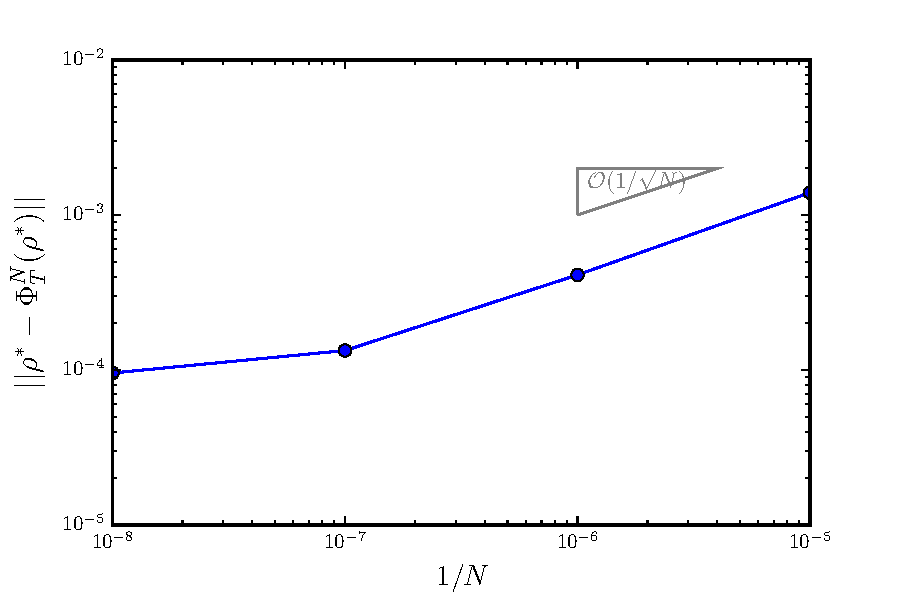
\includegraphics[width=0.56\linewidth]{/home/pieter/riskmodel/Problems/WeightedParticles/checkSystem/plots/Tolerance_on_NK-solution_converges_N-1}
\end{figure}
%The needed number of Newton iterations and the tolerance after convergence depend on the number of particles $N$ (\textit{left}). This best achieved tolerance converges to zero with  $\mathcal{O}(\frac{1}{\sqrt{N}})$


\end{frame}



\begin{frame} {Estimating $\Delta T$}
%Calculate steady states $\U^*$ by applying variance reduced Newton-Krylov-solver 

\begin{figure}
\centering
\includegraphics[width=0.7\linewidth]{/home/pieter/riskmodel/Problems/WeightedParticles/checkSystem/plots/Newton_states(DT)_it0}
\label{fig:Newton_states(DT)_it0}
\end{figure}
\end{frame}
\begin{frame} {Estimating $\Delta T$}
\begin{figure}
\centering
\includegraphics[width=0.7\linewidth]{/home/pieter/riskmodel/Problems/WeightedParticles/checkSystem/plots/Newton_states(DT)_it1}
\label{fig:Newton_states(DT)_it1}
\end{figure}
\end{frame}
\begin{frame} {Estimating $\Delta T$}
\begin{figure}
\centering
\includegraphics[width=0.7\linewidth]{/home/pieter/riskmodel/Problems/WeightedParticles/checkSystem/plots/Newton_states(DT)_it2}
\label{fig:Newton_states(DT)_it2}
\end{figure}
\end{frame}
\begin{frame}  {Estimating $\Delta T$}
\begin{figure}
\centering
\includegraphics[width=0.7\linewidth]{/home/pieter/riskmodel/Problems/WeightedParticles/checkSystem/plots/Newton_states(DT)_it3}

\label{fig:Newton_states(DT)_it3}
\end{figure}
\end{frame}
\begin{frame}  {Estimating $\Delta T$}
\begin{figure}
\centering
\includegraphics[width=0.7\linewidth]{/home/pieter/riskmodel/Problems/WeightedParticles/checkSystem/plots/Newton_states(DT)_it4}
\label{fig:Newton_states(DT)_it4}
\end{figure}
\end{frame}
\begin{frame}  {Estimating $\Delta T$}
\begin{figure}
\centering
\includegraphics[width=0.7\linewidth]{/home/pieter/riskmodel/Problems/WeightedParticles/checkSystem/plots/Newton_states(DT)_it5}
\label{fig:Newton_states(DT)_it5}
\end{figure}
\end{frame}
\begin{frame}  {Estimating $\Delta T$}
\begin{figure}
\centering
\includegraphics[width=0.7\linewidth]{/home/pieter/riskmodel/Problems/WeightedParticles/checkSystem/plots/Newton_states(DT)_it6}
\label{fig:Newton_states(DT)_it6}
\end{figure}
\end{frame}
\begin{frame}  {Estimating $\Delta T$}
\begin{figure}
\centering
\includegraphics[width=0.7\linewidth]{/home/pieter/riskmodel/Problems/WeightedParticles/checkSystem/plots/Newton_states(DT)_it7}
\label{fig:Newton_states(DT)_it7}
\end{figure}
\end{frame}
\begin{frame}  {Estimating $\Delta T$}
\begin{figure}
\centering
\includegraphics[width=0.7\linewidth]{/home/pieter/riskmodel/Problems/WeightedParticles/checkSystem/plots/Newton_states(DT)_it8}
\label{fig:Newton_states(DT)_it8}
\end{figure}


\end{frame}


\begin{frame}  {Estimating $\Delta T$}
\begin{figure}
\centering
\includegraphics[width=0.89\linewidth]{/home/pieter/riskmodel/Problems/WeightedParticles/checkSystem/plots/Newton_states_abs_bias_N1e6}

\end{figure}

\end{frame}

\begin{frame}   {Estimating $\Delta T$}
\begin{figure}
\centering
\includegraphics[width=0.82\linewidth]{/home/pieter/riskmodel/Problems/WeightedParticles/checkSystem/plots/Newton_states_abs_bias_N1e4_5_6_7}
\end{figure}
\end{frame}

\begin{frame} {Efficiency compared with direct simulation}
\begin{figure}
\centering
\includegraphics[width=0.9\linewidth]{/home/pieter/riskmodel/Problems/WeightedParticles/checkSystem/plots/bias_compare_Newton_direct}
\label{fig:bias_compare_Newton_direct}
\end{figure}

\end{frame}



%\begin{frame}{Bifurcation diagram}


%
%\begin{figure} % {Bifurcation diagram}
%
%%Increment the continuation parameter and solve a new problem using the previous solution as an initial guess
%
%\centering
%\includegraphics[width=0.9\linewidth]{/home/pieter/riskmodel/Problems/WeightedParticles/checkSystem/plots/bif_alpha}
%\label{fig:bifurcation}
%\end{figure}
%\end{frame}

\begin{frame}{Bifurcation diagram}

\begin{figure} % {Bifurcation diagram}

%Increment the continuation parameter and solve a new problem using the previous solution as an initial guess

\centering
\includegraphics[width=0.9\linewidth]{/home/pieter/riskmodel/Problems/WeightedParticles/checkSystem/plots/bifurcation_0}
\label{fig:bifurcation}
\end{figure}

\end{frame}

\begin{frame}{Bifurcation diagram}

\begin{figure} % {Bifurcation diagram}

%Increment the continuation parameter and solve a new problem using the previous solution as an initial guess

\centering
\includegraphics[width=0.9\linewidth]{/home/pieter/riskmodel/Problems/WeightedParticles/checkSystem/plots/bifurcation_1}
\label{fig:bifurcation}
\end{figure}

\end{frame}


\begin{frame}{Bifurcation diagram}

\begin{figure} % {Bifurcation diagram}

%Increment the continuation parameter and solve a new problem using the previous solution as an initial guess

\centering
\includegraphics[width=0.9\linewidth]{/home/pieter/riskmodel/Problems/WeightedParticles/checkSystem/plots/bifurcation_fin}
\label{fig:bifurcation}
\end{figure}

\end{frame}



\section{Research Plan}

\section{Other}


\begin{frame} {Courses}


\begin{block}{Contribution to Education}
\begin{itemize}
\item Exercises Analysis 1
\item Exercises Analysis 2
\end{itemize}
\end{block}

\begin{block}{Doctoral Training Programme}
\begin{itemize}
\item Seminar scientific integrity 
\item Teacher assistant training 
\item Science Communication and Outreach 
\end{itemize}
\end{block}

\begin{block}{Other courses}
\begin{itemize}
\item Functional Analysis
\end{itemize}
\end{block}
\end{frame}




%\cite{Garnier}
%\nocite{avitabile14}

%\begin{posterbox}[name=noisereducedjv, column=1, row=3, below=systemic, above=bottom]{References} %ofJacobian-vector-products}

%\renewcommand\refname{\vskip -0.4cm}
%\bibliographystyle{abbrv}
%\bibliography{biblio.bib}

\end{document}